\section{Thống kê mô tả}

\subsection{Các giá trị đặc trưng mẫu}

Để khảo sát các đặc trưng xu hướng trung tâm và độ phân tán của các thông số kỹ thuật GPU rời (tệp \texttt{gpus\_analysis.parquet} gồm $n = 2057$ quan trắc), nhóm sử dụng các chỉ số thống kê gồm: giá trị nhỏ nhất (\textbf{Min}), giá trị lớn nhất (\textbf{Max}), giá trị trung bình (\textbf{Mean}), độ lệch chuẩn (\textbf{SD}), trung vị (\textbf{Median}), tứ phân vị thứ nhất (\textbf{Q1}), tứ phân vị thứ ba (\textbf{Q3}) và khoảng tứ phân vị (\textbf{IQR}). Biến \texttt{core\_speed\_mhz} được loại khỏi tập phân tích chính do tỷ lệ khuyết dữ liệu cao và không giữ vai trò quyết định độc lập trong mô hình công suất.

Trong Python, các đại lượng này được tính toán thông qua thư viện \texttt{pandas} và \texttt{numpy}:

\begin{lstlisting}[language=Python]
import pandas as pd
import numpy as np

# Doc du lieu GPU da duoc lam sach va an danh muc hang khong co du lieu
df = pd.read_parquet("data/processed/gpus_analysis.parquet")
df['manufacturer'] = df['manufacturer'].cat.remove_unused_categories()

# Danh sach 6 bien dinh luong chinh
num_cols = [
    'max_power_w', 'process_nm', 'memory_bandwidth_gb_s',
    'memory_mb', 'tmus', 'texture_rate_per_watt'
]

# Tinh toan cac gia tri dac trung mau
stats_df = pd.DataFrame({
    'Min': df[num_cols].min(),
    'Max': df[num_cols].max(),
    'Mean': df[num_cols].mean(),
    'SD': df[num_cols].std(),
    'Median': df[num_cols].median(),
    'Q1': df[num_cols].quantile(0.25),
    'Q3': df[num_cols].quantile(0.75),
    'IQR': df[num_cols].quantile(0.75) - df[num_cols].quantile(0.25)
}).round(2)

print(stats_df)
\end{lstlisting}

Ý nghĩa chi tiết của 6 biến kỹ thuật định lượng đại diện cho GPU trong bài phân tích bao gồm:
\begin{itemize}\tightlist
    \item \texttt{max\_power\_w} \textbf{(Max Power -- Watt):} Công suất tiêu thụ điện năng tối đa của card đồ họa khi hoạt động ở mức tải cao nhất.
    \item \texttt{process\_nm} \textbf{(Process Size -- nm):} Kích thước tiến trình sản xuất bán dẫn của chip GPU (đơn vị nanomet). Tiến trình càng nhỏ thể hiện công nghệ sản xuất càng tiên tiến và tiết kiệm điện.
    \item \texttt{memory\_bandwidth\_gb\_s} \textbf{(Memory Bandwidth -- GB/s):} Băng thông bộ nhớ VRAM, phản ánh tốc độ truyền dữ liệu giữa bộ nhớ đồ họa và nhân GPU trong một giây.
    \item \texttt{memory\_mb} \textbf{(Memory Size -- MB):} Dung lượng bộ nhớ đồ họa VRAM (đơn vị Megabyte), cho biết khả năng lưu trữ dữ liệu hình ảnh, kết cấu (texture) của card.
    \item \texttt{tmus} \textbf{(Texture Mapping Units):} Số lượng đơn vị xử lý phủ vân bề mặt hình ảnh 3D trong cấu trúc phần cứng của GPU.
    \item \texttt{texture\_rate\_per\_watt} \textbf{(Texture Rate per Watt):} Tỷ lệ hiệu suất xử lý phủ vân bề mặt trên mỗi Watt công suất tiêu thụ, phản ánh hiệu suất năng lượng của GPU.
\end{itemize}

Bảng~\ref{tab:gpu_descriptive_stats} tổng hợp các giá trị đặc trưng thu được từ tập dữ liệu GPU sau tiền xử lý.

\begin{table}[H]
    \centering
    \footnotesize
    \setlength{\tabcolsep}{4.5pt}
    \caption{Các giá trị đặc trưng mẫu của các biến định lượng kỹ thuật GPU}
    \label{tab:gpu_descriptive_stats}
    \renewcommand{\arraystretch}{1.3}
    \resizebox{\linewidth}{!}{%
    \begin{tabular}{|l|c|c|c|c|c|c|c|c|}
        \hline
        \rowcolor{TableHead}
        \textbf{Tên biến} & \textbf{Min} & \textbf{Max} & \textbf{Mean} & \textbf{SD} & \textbf{Median} & \textbf{Q1} & \textbf{Q3} & \textbf{IQR} \\ \hline
        \texttt{max\_power\_w} (Watts) & 5.00 & 375.00 & 124.93 & 76.94 & 120.00 & 64.00 & 171.00 & 107.00 \\ \hline
        \texttt{process\_nm} (nm) & 14.00 & 150.00 & 30.93 & 13.63 & 28.00 & 28.00 & 40.00 & 12.00 \\ \hline
        \texttt{memory\_bandwidth\_gb\_s} (GB/s) & 4.00 & 547.20 & 144.86 & 110.73 & 112.20 & 57.70 & 224.00 & 166.30 \\ \hline
        \texttt{memory\_mb} (MB) & 128.00 & 16384.00 & 3063.13 & 2531.27 & 2048.00 & 1024.00 & 4096.00 & 3072.00 \\ \hline
        \texttt{tmus} & 4.00 & 256.00 & 76.58 & 57.33 & 64.00 & 32.00 & 120.00 & 88.00 \\ \hline
        \texttt{texture\_rate\_per\_watt} & 0.03 & 1.92 & 0.66 & 0.37 & 0.59 & 0.37 & 0.84 & 0.47 \\ \hline
    \end{tabular}%
    }
\end{table}

Bên cạnh đó, đối với biến phân loại định tính Hãng sản xuất (\texttt{manufacturer}) sau khi loại bỏ các hãng không có dữ liệu GPU rời trong mẫu (như Intel), bảng tần số và tần suất được tổng hợp ở Bảng~\ref{tab:freq_manufacturer}.

\begin{table}[H]
    \centering
    \small
    \caption{Bảng tần số và tần suất của biến Hãng sản xuất}
    \label{tab:freq_manufacturer}
    \renewcommand{\arraystretch}{1.25}
    \begin{tabular}{|l|c|c|c|}
        \hline
        \rowcolor{TableHead}
        \textbf{Hãng sản xuất} & \textbf{Số lượng mẫu (Tần số)} & \textbf{Tỷ lệ (\%)} & \textbf{Tỷ lệ tích lũy (\%)} \\ \hline
        Nvidia & 1186 & 57.66\% & 57.66\% \\ \hline
        AMD & 794 & 38.60\% & 96.26\% \\ \hline
        ATI & 77 & 3.74\% & 100.00\% \\ \hline
        \textbf{Tổng cộng} & \textbf{2057} & \textbf{100.00\%} & -- \\ \hline
    \end{tabular}
\end{table}

\subsection{Đồ thị mô tả dữ liệu}

Nhằm quan sát trực quan dạng phân phối của biến mục tiêu \texttt{max\_power\_w}, so sánh sự khác biệt công suất giữa các phân khúc thiết bị (\texttt{segment}) và đánh giá mối tương quan giữa các thông số phần cứng, nhóm trực quan hóa dữ liệu bằng ba đồ thị dưới đây.

\subsubsection{Biểu đồ tần suất công suất tiêu thụ tối đa (Histogram)}

Mã nguồn Python vẽ biểu đồ tần suất Histogram cho biến \texttt{max\_power\_w} trên thang đo gốc (Watts) và thang đo Logarithm tự nhiên ($\ln$):

\begin{lstlisting}[language=Python]
# Graph 1: Histogram Max_Power (Goc vs Log)
fig, axes = plt.subplots(1, 2, figsize=(11, 4.5))
sns.histplot(df['max_power_w'], kde=True, ax=axes[0], color='skyblue')
axes[0].set_title('Phan bo Max_Power (Watts)')

sns.histplot(np.log(df['max_power_w']), kde=True, ax=axes[1], color='salmon')
axes[1].set_title('Phan bo ln(Max_Power)')
plt.tight_layout()
plt.savefig(CURRENT_DIR / "histogram_max_power.png", dpi=300)
plt.close()
\end{lstlisting}

\begin{figure}[H]
    \centering
    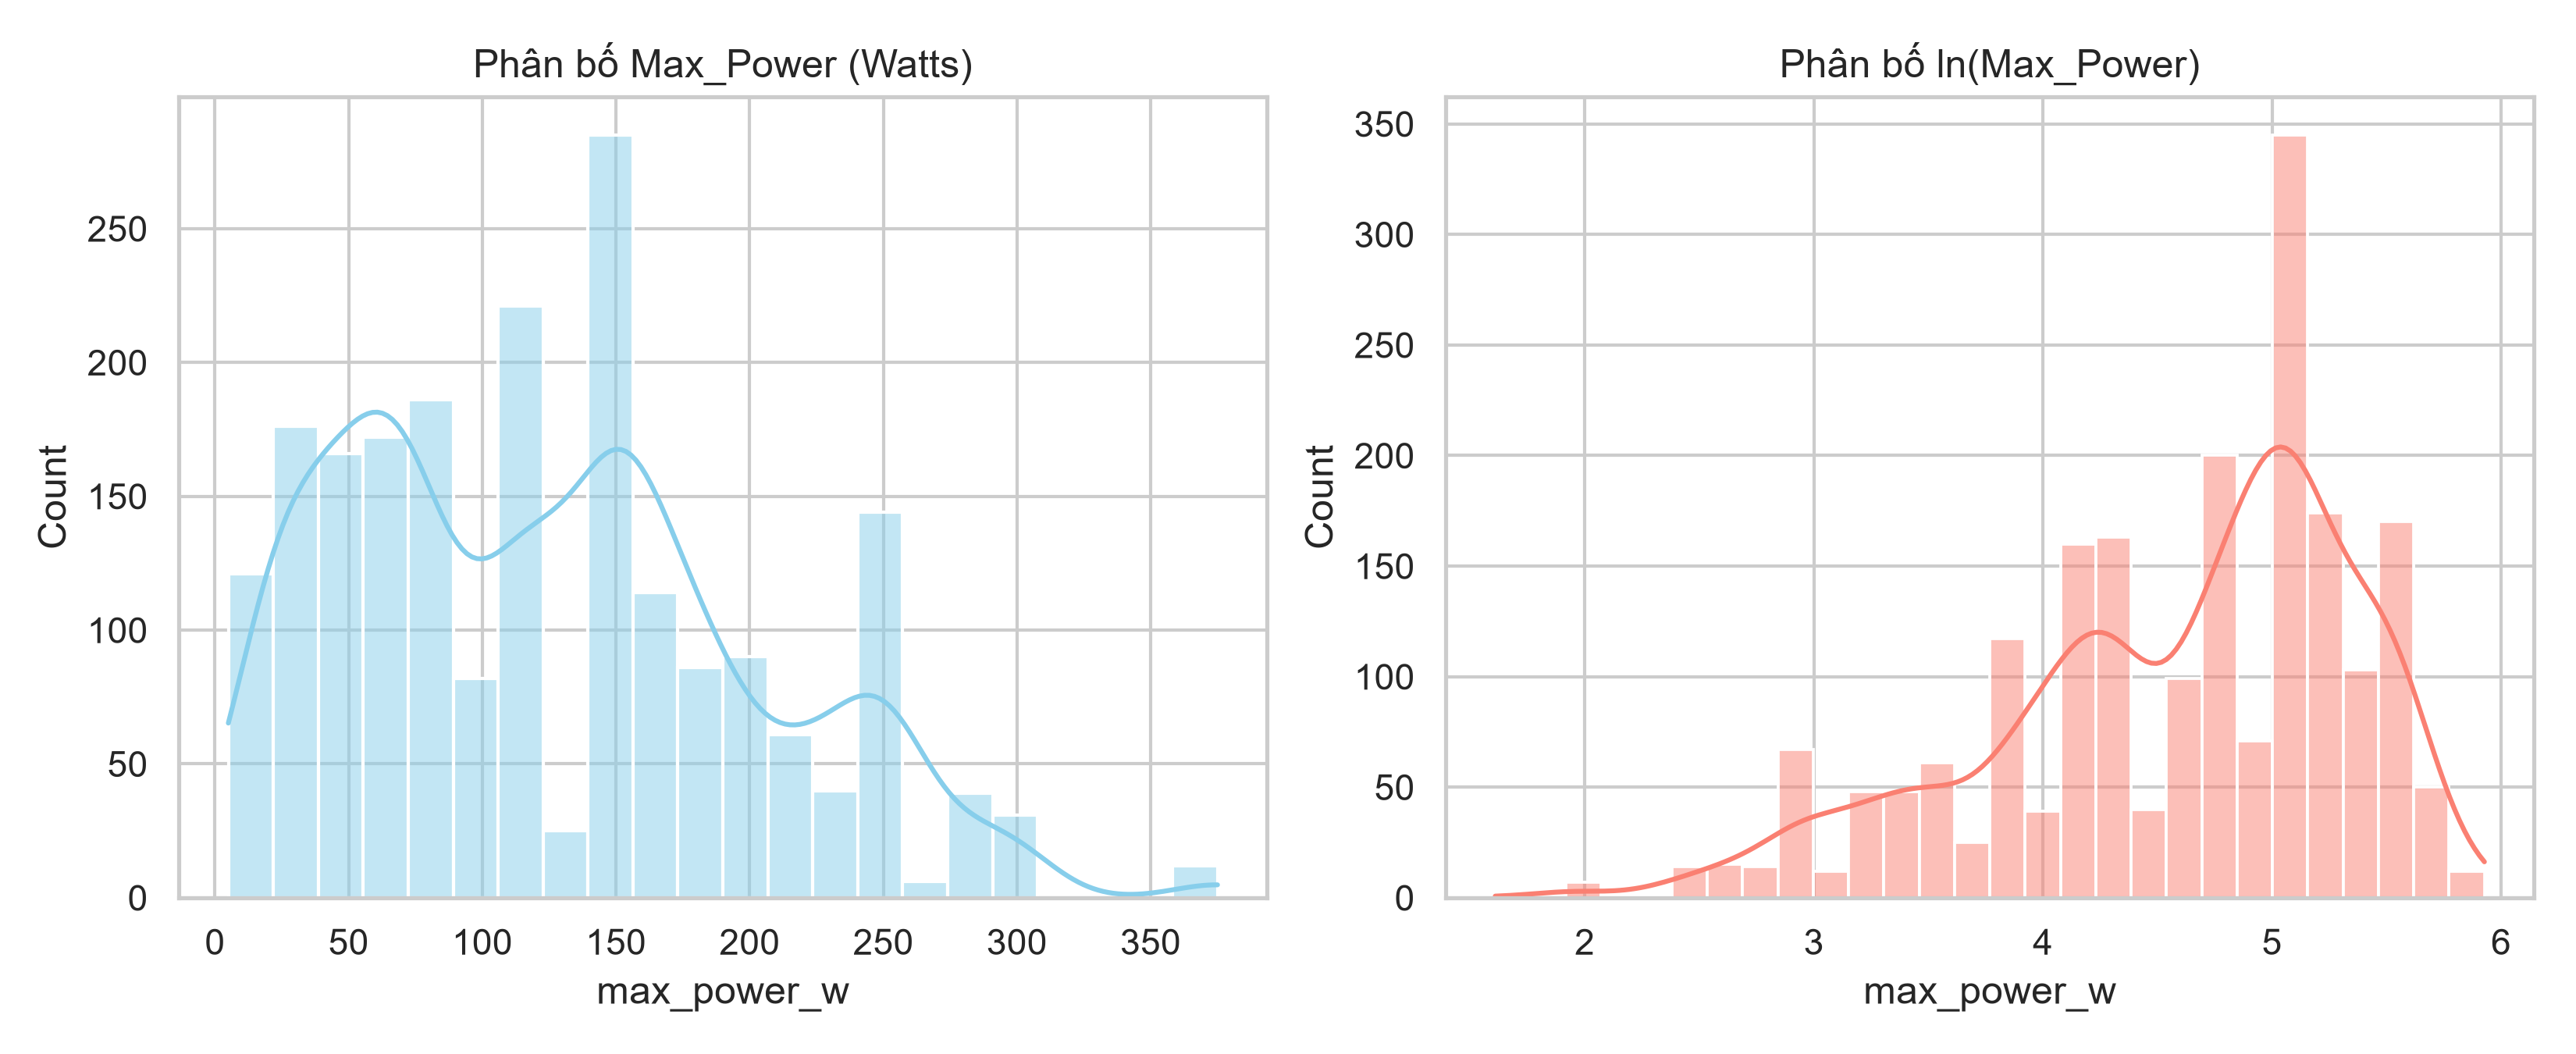
\includegraphics[width=0.88\textwidth]{figures/histogram_max_power.png}
    \caption{Biểu đồ phân bố công suất tiêu thụ tối đa \texttt{max\_power\_w} (Thang đo gốc Watts và thang đo Logarithm)}
    \label{fig:hist_max_power}
\end{figure}

\textbf{Nhận xét biểu đồ Histogram:}
\begin{itemize}\tightlist
    \item \textbf{Trên thang đo gốc (Watts):} Phân bố của \texttt{max\_power\_w} lệch phải rõ rệt (đỉnh tập trung về phía bên trái), cho thấy phần lớn các mẫu GPU nằm ở phân khúc công suất thấp và phổ thông (trung vị đạt $120.00\text{ W}$ và $75\%$ số mẫu có công suất từ $171.00\text{ W}$ trở xuống, khoảng tứ phân vị $\text{IQR} = 107.00\text{ W}$). Phần đuôi kéo dài sang bên phải đại diện cho nhóm card đồ họa cao cấp có mức tiêu thụ điện năng lớn từ $250\text{ W}$ đến $375\text{ W}$.
    \item \textbf{Sau khi biến đổi Logarithm ($\ln$):} Dữ liệu được dàn trải đều hơn, giảm thiểu độ lệch phải và co cụm lại quanh vùng trung tâm từ $4.0$ đến $5.5$, giúp phân bố tiệm cận dạng cân đối hơn để phục vụ các bước kiểm định và hồi quy tuyến tính.
\end{itemize}

\subsubsection{Biểu đồ hộp so sánh công suất tiêu thụ (Boxplot)}

Mã nguồn Python vẽ biểu đồ hộp Boxplot so sánh phân bố công suất \texttt{max\_power\_w} giữa hai phân khúc thiết bị Desktop và Laptop (\texttt{segment}) theo từng Hãng sản xuất (\texttt{manufacturer}):

\begin{lstlisting}[language=Python]
# Graph 2: Boxplot Desktop vs Laptop
plt.figure(figsize=(8, 4.5))
sns.boxplot(x='manufacturer', y='max_power_w', hue='segment', data=df, palette='Set2')
plt.title('So sanh Max_Power giua Desktop va Laptop')
plt.tight_layout()
plt.savefig(CURRENT_DIR / "boxplot_max_power.png", dpi=300)
plt.close()
\end{lstlisting}

\begin{figure}[H]
    \centering
    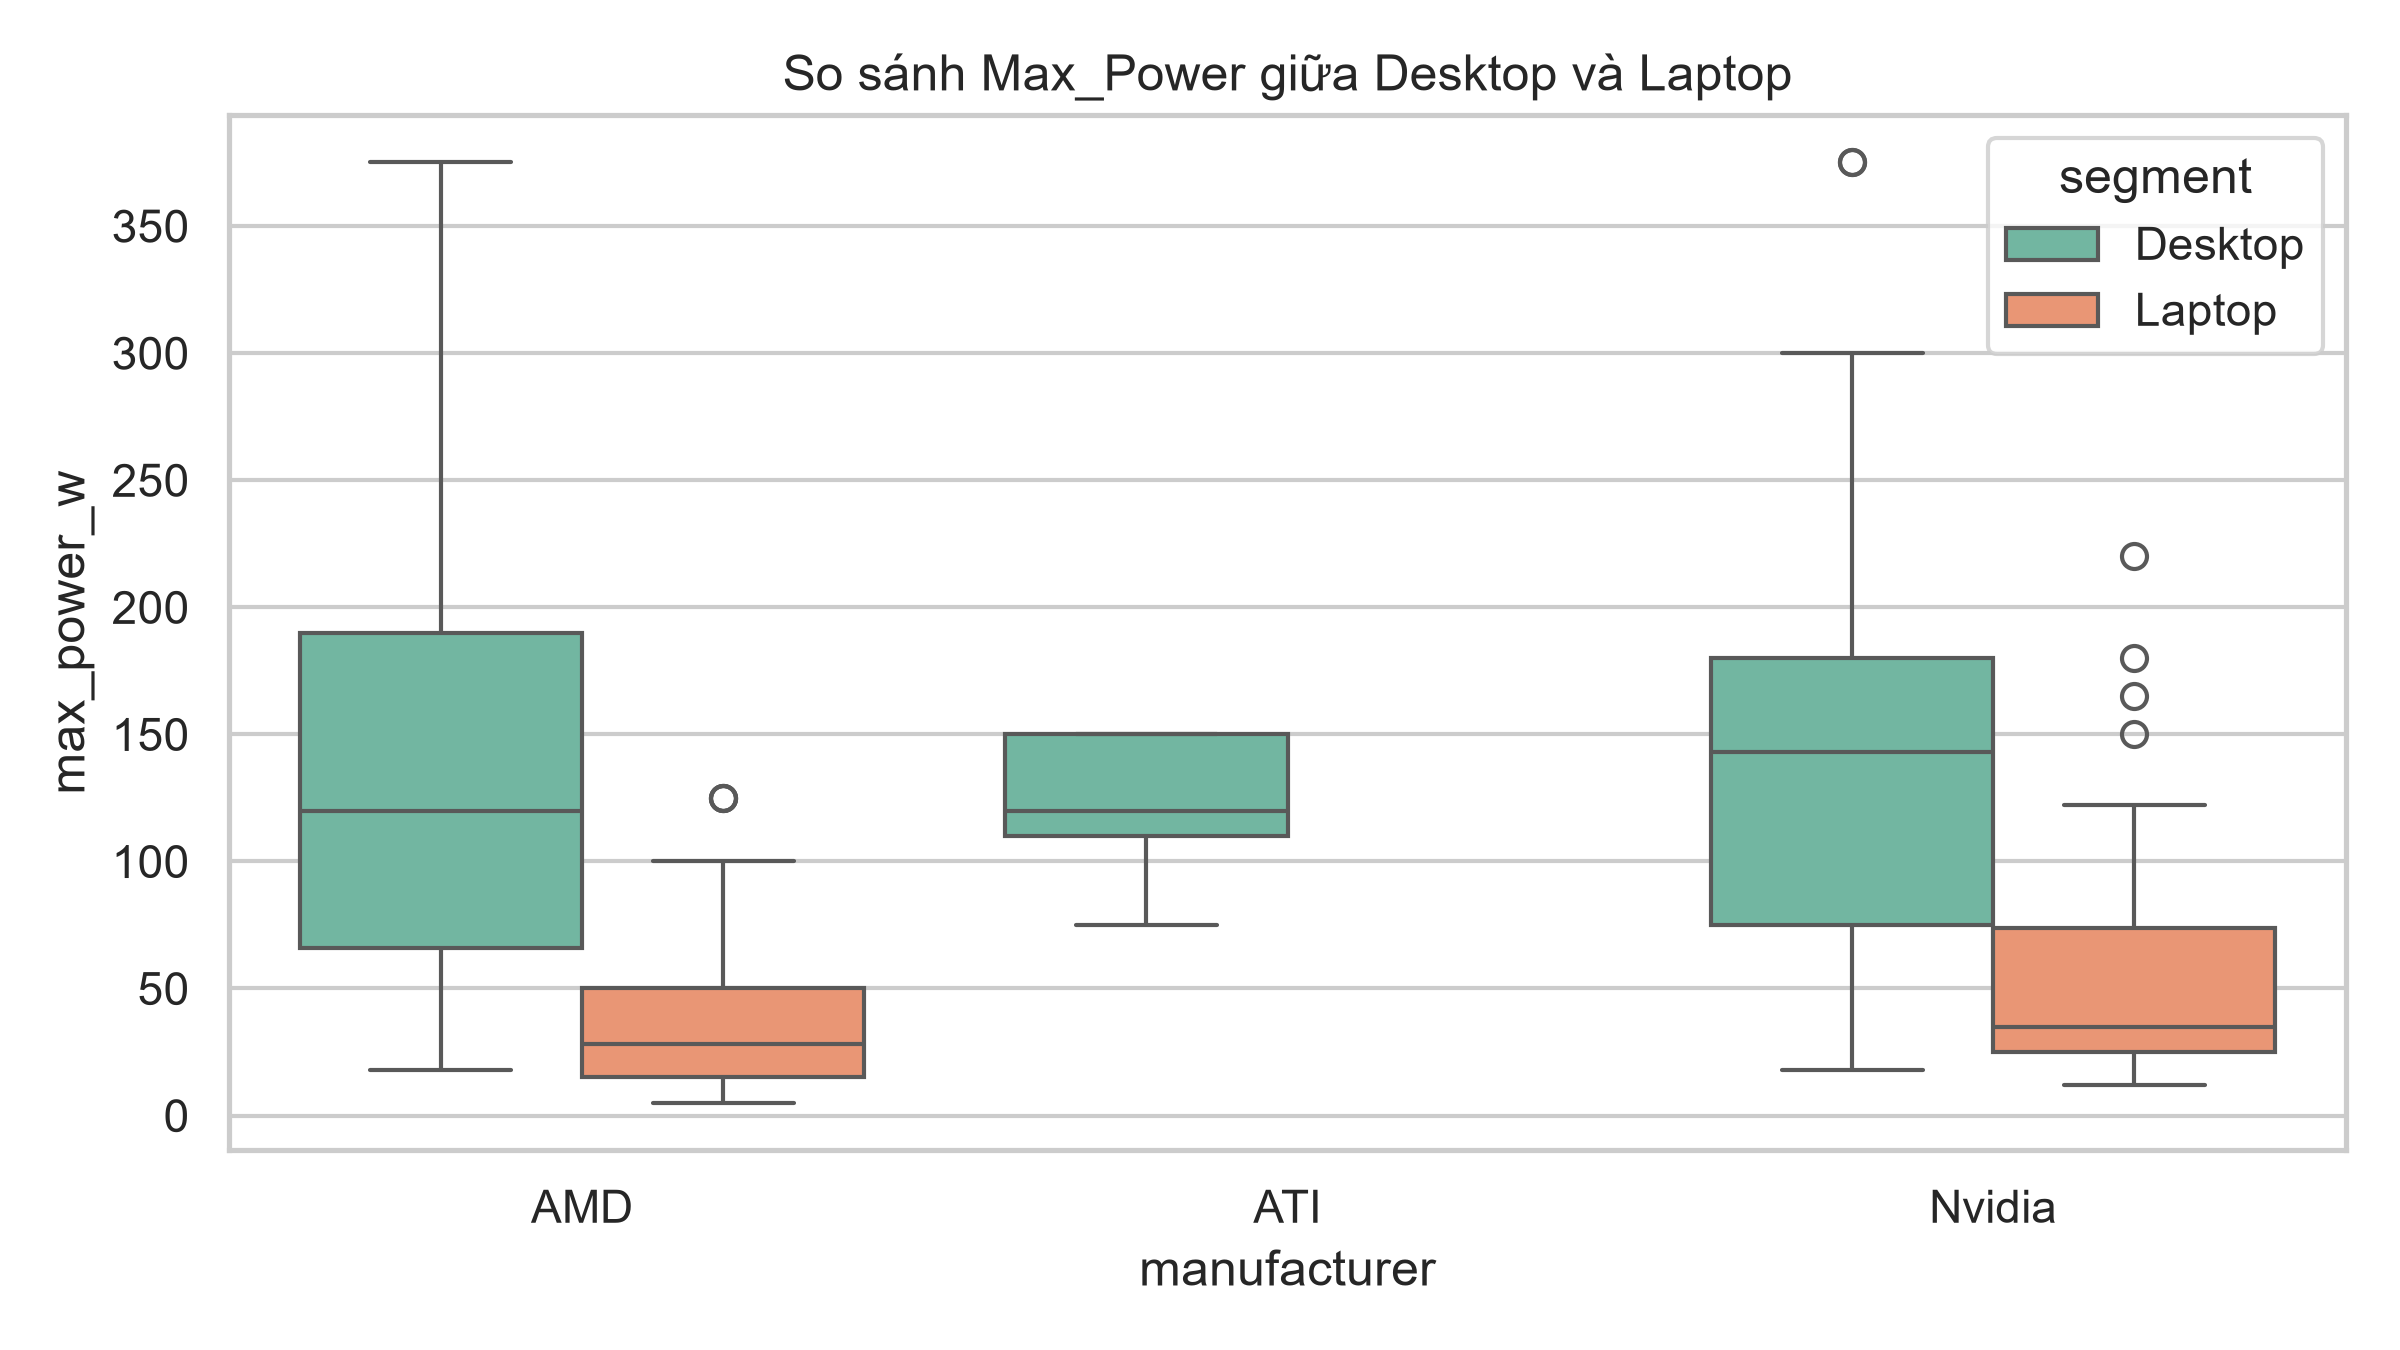
\includegraphics[width=0.82\textwidth]{figures/boxplot_max_power.png}
    \caption{Biểu đồ hộp so sánh công suất \texttt{max\_power\_w} theo Hãng sản xuất và Phân khúc Desktop/Laptop}
    \label{fig:boxplot_max_power}
\end{figure}

\textbf{Nhận xét biểu đồ Boxplot:}
\begin{itemize}\tightlist
    \item \textbf{Theo phân khúc thiết bị:} Ở cả AMD và Nvidia, phân khúc Laptop có mức trung vị (khoảng $28\text{--}35\text{ W}$) và khoảng tứ phân vị $\text{IQR}$ nhỏ hơn đáng kể so với phân khúc Desktop (trung vị khoảng $120\text{--}143\text{ W}$), phản ánh giới hạn nghiêm ngặt về nguồn cấp và tản nhiệt trên thiết bị di động. Riêng hãng ATI chỉ ghi nhận các mẫu thuộc phân khúc Desktop (do thương hiệu này đã được AMD sáp nhập và ngừng phát triển các dòng chip di động thế hệ mới).
    \item \textbf{Theo hãng sản xuất và giá trị ngoại lệ:} AMD và Nvidia có dải công suất trải rộng từ các dòng phổ thông đến cao cấp (lên tới $375\text{ W}$). Xuất hiện một số điểm ngoại lệ phía trên rào chắn $Q_3 + 1.5\text{IQR}$ ở phân khúc Laptop của AMD, Nvidia và phân khúc Desktop của Nvidia, đại diện cho các mẫu GPU hiệu năng cao dành cho máy trạm hoặc laptop chơi game chuyên dụng.
\end{itemize}

\subsubsection{Biểu đồ ma trận hệ số tương quan (Correlation Heatmap)}

Đoạn mã Python tính toán ma trận hệ số tương quan Pearson ($r_{XY}$) giữa 6 biến định lượng và trực quan hóa bằng biểu đồ nhiệt (Heatmap):

\begin{lstlisting}[language=Python]
# Graph 3: Correlation Matrix Heatmap
plt.figure(figsize=(7, 5))
sns.heatmap(df[num_cols].corr(), annot=True, fmt=".2f", cmap='coolwarm', vmin=-1, vmax=1)
plt.title('Ma tran he so tuong quan Pearson')
plt.tight_layout()
plt.savefig(CURRENT_DIR / "correlation_matrix.png", dpi=300)
plt.close()
\end{lstlisting}

\begin{figure}[H]
    \centering
    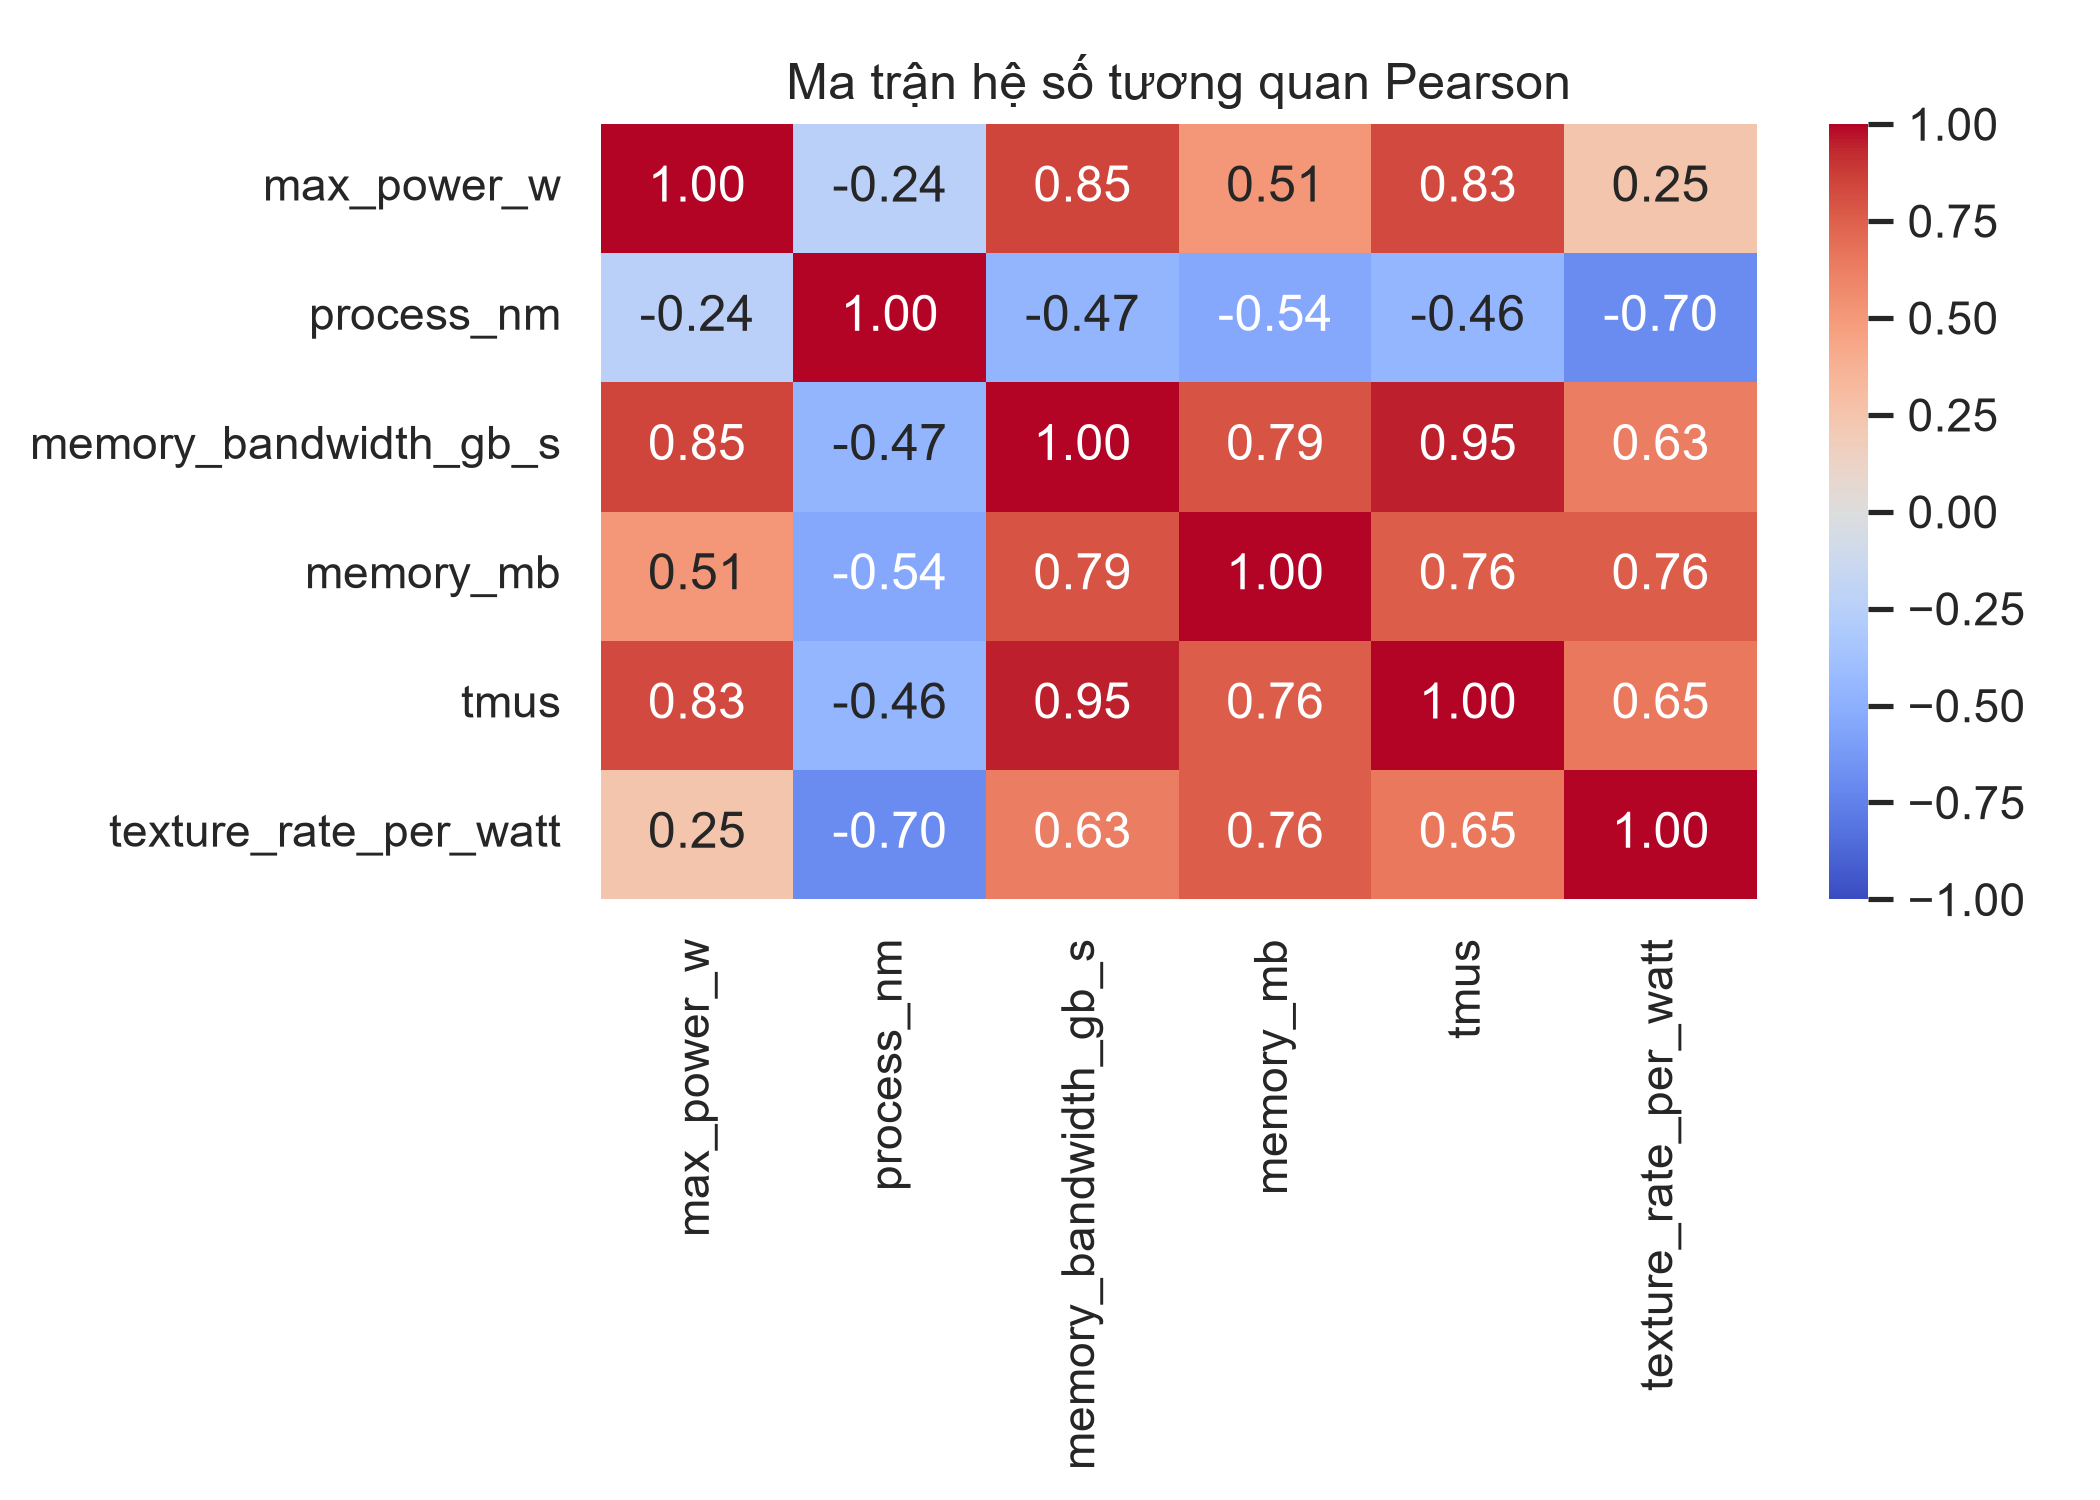
\includegraphics[width=0.76\textwidth]{figures/correlation_matrix.png}
    \caption{Ma trận hệ số tương quan Pearson giữa 6 biến kỹ thuật định lượng}
    \label{fig:corr_matrix}
\end{figure}

\textbf{Nhận xét mối liên hệ tương quan:}
\begin{itemize}\tightlist
    \item \textbf{Tương quan với biến mục tiêu \texttt{max\_power\_w}:} Công suất tiêu thụ tối đa có tương quan thuận rất mạnh với Băng thông bộ nhớ \texttt{memory\_bandwidth\_gb\_s} ($r = 0.85$) và Số đơn vị xử lý phủ vân bề mặt \texttt{tmus} ($r = 0.83$), cùng mức tương quan trung bình với Dung lượng bộ nhớ \texttt{memory\_mb} ($r = 0.51$). Điều này cho thấy các card đồ họa có quy mô nhân xử lý lớn và băng thông bộ nhớ cao đòi hỏi công suất cấp nguồn lớn hơn rõ rệt.
    \item \textbf{Tương quan giữa các biến kỹ thuật và hiệu suất năng lượng:} Kích thước tiến trình bán dẫn \texttt{process\_nm} có tương quan nghịch mạnh với Hiệu suất năng lượng \texttt{texture\_rate\_per\_watt} ($r = -0.70$) và Dung lượng bộ nhớ \texttt{memory\_mb} ($r = -0.54$), chứng minh việc thu nhỏ tiến trình sản xuất giúp nâng cao đáng kể hiệu năng xử lý trên mỗi Watt điện năng tiêu thụ. Bên cạnh đó, \texttt{tmus} và \texttt{memory\_bandwidth\_gb\_s} có tương quan thuận rất chặt chẽ ($r = 0.95$), phản ánh sự cân đối đồng bộ giữa năng lực tính toán của nhân đồ họa và tốc độ truyền tải bộ nhớ.
\end{itemize}

\subsection{Tổng kết đặc điểm dữ liệu}

Từ các kết quả thống kê mô tả và trực quan hóa trên tập dữ liệu $n = 2057$ GPU rời, có thể rút ra những đặc điểm chính sau:
\begin{itemize}\tightlist
    \item \textbf{Quy mô và cơ cấu mẫu:} Dữ liệu tập trung chủ yếu vào hai nhà sản xuất lớn là Nvidia ($57.66\%$) và AMD ($38.60\%$), chiếm hơn $96\%$ tổng số mẫu nghiên cứu; phần còn lại thuộc về ATI ($3.74\%$).
    \item \textbf{Đặc điểm phân phối công suất:} Biến mục tiêu \texttt{max\_power\_w} biến thiên rộng từ $5.00\text{ W}$ đến $375.00\text{ W}$ với phân phối lệch phải ($\text{Mean} = 124.93\text{ W} > \text{Median} = 120.00\text{ W}$, $\text{IQR} = 107.00\text{ W}$). Việc biến đổi sang thang đo $\ln(\texttt{max\_power\_w})$ giúp phân bố dữ liệu cân đối hơn, phù hợp cho các phân tích suy diễn tiếp theo.
    \item \textbf{Sự phân hóa theo phân khúc và thông số phần cứng:} Công suất tiêu thụ có sự phân tầng rõ rệt giữa hai nhóm thiết bị Desktop và Laptop, đồng thời chịu tác động tuyến tính thuận rất mạnh từ băng thông bộ nhớ ($r = 0.85$) và số lượng đơn vị TMUs ($r = 0.83$).
\end{itemize}
